\documentclass[%
    % final,
	pdftex,
	oneside,			% Einseitiger Druck (oneside) oder zweiseitig (twoside)
	headings=openright,	% Kapitelanfänge immer auf rechter Seite (bei zweiseitig)
	cleardoublepage=empty,	% Leere Vakatseiten
	11pt,				% Schriftgroesse
	parskip=half,		% Halbe Zeile Abstand zwischen Absätzen (half).
%	topmargin = 10pt,	% Abstand Seitenrand (Std:1in) zu Kopfzeile [laut log: unused]
	headheight = 20pt,	% Höhe der Kopfzeile
%	headsep = 30pt,	% Abstand zwischen Kopfzeile und Text Body  [laut log: unused]
	headsepline,		% Linie nach Kopfzeile.
	% footsepline,		% Linie vor Fusszeile.
	footheight = 10pt,	% Höhe der Fusszeile
	abstracton,		% Abstract Überschriften
	DIV=calc,		% Satzspiegel berechnen
	headinclude=false,	% Kopfzeile nicht in den Satzspiegel einbeziehen
	footinclude=false,	% Fußzeile nicht in den Satzspiegel einbeziehen
	listof=totoc,		% Abbildungs-/ Tabellenverzeichnis im Inhaltsverzeichnis darstellen
	toc=bibliography,	% Literaturverzeichnis im Inhaltsverzeichnis darstellen
	pointlessnumbers,
	fleqn,
	chapterprefix=false,
  appendixprefix=false,
	% bibliography=openstyle
]{scrreprt}

\usepackage[base]{babel}

%!TEX root = ../main.tex

% PDF Einstellungen
\usepackage[%
	pdfcreator={pdflatex, LaTeX with KOMA-Script},
	pdfpagemode=UseOutlines, 		% Beim Oeffnen Inhaltsverzeichnis anzeigen
	pdfdisplaydoctitle=true, 		% Dokumenttitel statt Dateiname anzeigen.
	%hidelinks,						% entfernt Umrandung von verlinkten Stellen, ohne Verlinkung zu löschen
]{hyperref}

% (Farb-)einstellungen für die Links im PDF
\hypersetup{%
	colorlinks=true, 		% Aktivieren von farbigen Links im Dokument
	linkcolor=ees_blue, 	% Farbe festlegen
	citecolor=ees_blue,
	filecolor=ees_blue,
	menucolor=ees_blue,
	urlcolor=ees_blue,
	linktocpage=false, 		% Nicht der Text sondern die Seitenzahlen in Verzeichnissen klickbar
	bookmarksnumbered=true 	% Überschriftsnummerierung im PDF Inhalt anzeigen.
}

\usepackage[table,dvipsnames]{xcolor}

\definecolor{lightgray}{RGB}{227, 227, 227}
\definecolor{darkgray}{RGB}{100, 100, 100}
\definecolor{purple}{rgb}{0.65, 0.12, 0.82}
\definecolor{schaeffler}{RGB}{0, 137, 61}
\definecolor{dark-green}{RGB}{0, 110, 93}
\definecolor{middle-green}{RGB}{115, 161, 149}
\definecolor{light-green}{RGB}{199, 222, 160}

\definecolor{pie1}{RGB}{115, 161, 149}
\definecolor{pie2}{RGB}{192, 198, 191}
\definecolor{pie3}{RGB}{135, 135, 135}
\definecolor{pie4}{RGB}{29, 155, 178}
\definecolor{pie5}{RGB}{182, 186, 194}
\definecolor{pie6}{RGB}{161, 200, 97}
\definecolor{pie7}{RGB}{67, 99, 91}
\definecolor{pie8}{RGB}{112, 123, 110}
\definecolor{pie9}{RGB}{113, 113, 113}

\definecolor{ees_blue}{RGB}{0, 112, 192}
\definecolor{ees_yellow}{RGB}{213, 223, 0}
\definecolor{ees_green}{RGB}{0, 166, 74}
\definecolor{ees_red}{RGB}{192, 0, 0}
\definecolor{ees_lightblue}{RGB}{0, 176, 240}
\definecolor{ees_black}{RGB}{0, 0, 0}

\usepackage[left=2.5cm,right=4.5cm,top=2.5cm,bottom=2.5cm,foot=.5cm]{geometry}
\usepackage{lipsum}
\usepackage{charter}

\usepackage{tikz}
\usetikzlibrary{positioning}
\usetikzlibrary{external}
\usepackage{circuitikzgit}
%!TEX root = ../main.tex

\usetikzlibrary{positioning,calc,shapes,arrows,shapes.multipart}

% circuitikz: creating a bus
\tikzset{bus/.style={fullgeneric, %
        bipoles/fullgeneric/width=0.02, bipoles/fullgeneric/height=#1
    },
    bus/.default=3
}
\newcommand{\bushere}[3]{% length, text above, text below
    % optional arguments do not work in paths
    %
    % starting point; draw an edge and then two nodes
    % save the position
    coordinate(tmp)
    % go up and do an edge down
    ++(0,#1) node[anchor=base]{#2} edge[ultra thick] ++(0,{-2*#1})
    % edges do not move the current point, go down to position the node
    ++(0,{-2*#1}) node[below]{#3}
    % go back to where we started
    (tmp)
}

% program plan
\tikzset{
   papDecision/.style = {
         diamond,
         draw, 
         text width = 20 mm, 
         align = center, 
         text badly centered,
         inner sep = 1 pt,
         font=\ttfamily\footnotesize,
         %line width = 1,
         minimum width = 30mm,
         minimum height = 7mm,
      },
   papStart/.style = {
         rectangle,
         draw, 
         align = center, 
         text width = 3cm, 
         text badly centered,
         inner sep = 4 pt,
         rounded corners=10pt,
         font=\ttfamily\footnotesize,
         %line width = 1,
         minimum width = 30mm,
         minimum height = 7mm,
      },
   papEnd/.style = {
         rectangle,
         draw, 
         align = center, 
         text width = 3cm, 
         text badly centered,
         inner sep = 4 pt,
         rounded corners=10pt,
         font=\ttfamily\footnotesize,
         %line width = 1,
         minimum width = 30mm,
         minimum height = 7mm,
      },
   papData/.style = {
         trapezium,
         draw, 
         align = center, 
         text width = 20 mm, 
         text badly centered,
         inner sep = 4 pt,
         trapezium left angle=70,
         trapezium right angle=110,
         font=\ttfamily\footnotesize,
         %line width = 1,
         minimum width = 30mm,
         minimum height = 7mm,
      },
   papPredProc/.style = {
         draw,
         rectangle split,
         rectangle split horizontal,
         rectangle split parts = 3,
         rectangle split empty part width=-8pt,
         align = center, 
 %       text width = 4.5 em, 
         text badly centered,
 %        inner sep = 4 pt,
         font=\ttfamily\footnotesize,
         %line width = 1,
         minimum width = 30mm,
         minimum height = 7mm,
      },
   papProcess/.style = {
         rectangle,
         draw,
         align = center, 
         text width = 3cm, 
         text badly centered,
         %inner sep = 2 pt,
         font=\ttfamily\footnotesize,
         %line width = 1,
         minimum width = 30mm,
         minimum height = 7mm,
      },
   papLine/.style = {
         draw,
         -stealth,
         font=\ttfamily\footnotesize,
         %line width = 1,
      },
}
\newcommand{\papYes}{ja}
\newcommand{\papNo}{nein}
\usetikzlibrary{arrows.meta}
\usepackage{pgf-umlcd}

\tikzexternalize[prefix=images/]

% Use follwing command for compiling in Terminal
% pdflatex -synctex=1 -interaction=nonstopmode --shell-escape external-pictures.tex


\pagestyle{empty}
\usetikzlibrary{shapes,arrows,positioning,calc}

\renewcommand{\umltextcolor}{ees_black}
\renewcommand{\umlfillcolor}{ees_green!10}
\renewcommand{\umldrawcolor}{ees_green!90}

\begin{document}

\listoffigures

\chapter{Grids}

\lipsum[2]

\vspace{1cm}

% \begin{tikzpicture}
%     % \vspace{10cm}
%     \begin{circuitikz}[european, scale=.9, smallR/.style={resistor,resistors/scale=.7}]
%         \draw (0,0) node[oscillator, anchor=east, name=gen]{} --(.5,0)
%         to[L, name=X_g] ++(2,0) coordinate(f1)
%         % \bushere{1}{$\underline{E}_\mathrm{T}'$}{}
%         % to[oosourcetrans,prim=delta,sec=wye] ++(2,0)
%         \bushere{2}{}{} coordinate(b1) ++(0,-1) -- ++(.25,0) -- coordinate(f2) ++(1.75,0)
%         to[L, name=X_l3] ++(1,0) -- ++(1.5,0) ++(0,1)
%         \bushere{2}{$E_\mathrm{ibb}~\angle~0^{\circ}$}{} ++(0,1) coordinate(b2) ++(0,-1) coordinate(b3) -- ++(.75,0) coordinate(f3) -- ++(.75,0) to[L, name=X_ibb] ++(1,0) -- ++(1,0)
%         node[gridnode, anchor=left, name=ib]{};
    
%         % draw other resistances
%         \draw (b1) ++(0,1) -- ++(.5,0) to[L, name=X_l1] (b2);
%         \draw (b1) -- ++(.5,0) to[L, name=X_l2] (b3);
%         % \draw[line width=2pt] (2.25,1) -- (2.25,-1);
%         % \draw[line width=2pt] (4.75,1) -- (4.75,-1);
%         % \draw[line width=2pt] (8.25,1) -- (8.25,-1);
    
%         % labels for the resistors
%         \node[above=6pt] at (X_g) {$X_\mathrm{g}'$};
%         \node[above=6pt] at (X_ibb) {$X_\mathrm{ibb}$};
%         \node[above=6pt] at (X_l1) {$3~X_\mathrm{l}$};
%         % \node[below=6pt] at (X_l2) {$X_\mathrm{l}$};
%         % \node[below=6pt] at (X_l3) {$X_\mathrm{l}$};
    
%         % pole voltages and angles
%         \path[->] (-1.2,.5) edge [bend right] node[left=6pt]{$E_\mathrm{p}~\angle~\delta$} (-1.2,-.5);
%         % \path[->] (ib) ++(.8,.5) edge [bend left] node[right=6pt]{$E_\mathrm{ibb}~\angle~0^{\circ}$} ++(0,-1);
    
%         % faults
%         % \draw[-Stealth, very thick, red] (f1) ++(0,-.5) -- ++(-.15,-.45) -- ++(.3,.2) -- ++(-.2,-.6) coordinate(f1_text);
%         % \node[below, red] at (f1_text) {\scriptsize fault 1};
%         % \draw[-Stealth, very thick, red] (f2) ++(0,.3) -- ++(-.15,-.45) -- ++(.3,.2) -- ++(-.2,-.6) coordinate(f2_text);
%         % \node[below, red, align=center] at (f2_text) {\scriptsize Fehler 2/3};
%         % \draw[-Stealth, very thick, red] (f3) ++(0,.3) -- ++(-.15,-.45) -- ++(.3,.2) -- ++(-.2,-.6) coordinate(f3_text);
%         % \node[below, red] at (f3_text) {\scriptsize Fehler 1};
%     \end{circuitikz}
% \end{tikzpicture}


\vspace{2cm}
\tikzsetnextfilename{sm_load_model.pdf}
\begin{figure}[htb]
    \begin{tikzpicture}[european, scale=.9, smallR/.style={resistor,resistors/scale=.7}]
        % \draw [help lines] (-1,-5) grid (15,5);
        \small
        \draw (0,0) node[oscillator, anchor=east, name=gen]{} --(.5,0)
        to ++(.5,0) \bushere{1}{}{Bus 2}
        to[oosourcetrans] ++(2,0) 
        \bushere{1}{}{Bus 1} -- ++(1.5,0) coordinate(line) -- ++(1.5,0)
        \bushere{2}{}{Bus 0} coordinate(b0);
        \draw (b0) ++(0,1) -- ++(1,0) \loadside{Load 1}{1}{0};
        \draw (b0) ++(0,-1) -- ++(1,0) \loadside{Load 2}{1}{0} ++(1,0);
    \end{tikzpicture}
    \caption{Single line network with two loads}
\end{figure}

\tikzsetnextfilename{smib_model.pdf}
\begin{figure}[htb]
    \begin{tikzpicture}[european, scale=.9, smallR/.style={resistor,resistors/scale=.7}]
        % \draw [help lines] (-1,-5) grid (15,5);
        \draw (0,0) node[oscillator, anchor=east, name=gen]{} --(.5,0)
        to ++(.5,0) \bushere{1}{}{Bus 2}
        to[oosourcetrans] ++(2,0) 
        \bushere{1}{}{Bus 1} -- ++(3,0) coordinate(line) -- ++(3,0)
        \bushere{1}{}{Bus 0}
        -- ++(1,0) node[gridnode, anchor=left, name=ib]{};
    \end{tikzpicture}
    \caption{SMIB model}
\end{figure}

\tikzsetnextfilename{smib_model_with_load.pdf}
\begin{figure}[htb]
    \begin{tikzpicture}[european, scale=.9, smallR/.style={resistor,resistors/scale=.7}]
        % \draw [help lines] (-1,-5) grid (15,5);
        \draw (0,0) node[oscillator, anchor=east, name=gen]{} --(.5,0)
        to ++(.5,0) \bushere{1}{}{Bus 2}
        to[oosourcetrans] ++(2,0) coordinate(trafo_b1) ++(0,-0.5)
        \bushere{1.5}{}{Bus 1} ++(0,-0.5) -- ++(1,0) \loadside{Load 1}{1}{0};
        \draw (trafo_b1) -- ++(3,0) coordinate(line) -- ++(3,0)
        \bushere{1}{}{Bus 0}
        -- ++(1,0) node[gridnode, anchor=left, name=ib]{};
    \end{tikzpicture}
    \caption{SMIB model with additional load}
\end{figure}

\tikzsetnextfilename{4bus3load_model_random.pdf}
\begin{figure}[htb]
    \begin{tikzpicture}[european, scale=.9, smallR/.style={resistor,resistors/scale=.7}]
        % \draw [help lines] (-5,-10) grid (5,0);
        \draw (0,0) node[oscillator, anchor=south, name=gen]{} --(0,-0.5)
        to ++(0,-0.5) \qbushere{2}{}{} ++(-1,0) coordinate(trafo)
        to[oosourcetrans] ++(0,-3)
        \qbushere{1}{}{} coordinate(b2) ++(.25,0) |- ++(2,-1) \bushere{1}{}{} -- ++(1,0) \loadhanging{Load 3}{0}{-.5};
        \draw (b2) ++(-.25,0) |- ++(-2,-1) \bushere{1}{}{} -- ++(-1,0) \loadhanging{Load 2}{0}{-.5};
        \draw (trafo) ++(2,0) \loadhanging{Load 1}{0}{-.5};
    \end{tikzpicture}
    \caption{Random network with three loads on multiple voltage levels}
\end{figure}

% \begin{figure}[htb]
%     \begin{circuitikz}[european, scale=.9, smallR/.style={resistor,resistors/scale=.7}]
%         \small
%         \node [oscillator, anchor=east](gen1){};
%         \node [gridnode, anchor=left](ibb){};
    
%         \draw (gen1) -- ++(1,0) \bushere{1}{}{} ++( 1,0) to[oosourcetrans] -- (ibb);
%         \draw (0,0) node[oscillator, anchor=east, name=gen]{} --(.5,0)
%         to ++(.5,0) \bushere{1}{}{Bus 2}
%         to[oosourcetrans] ++(2,0) 
%         \bushere{1}{}{Bus 1} -- ++(3,0) coordinate(line) -- ++(3,0)
%         \bushere{1}{}{Bus 0}
%         -- ++(1,0) node[gridnode, anchor=left, name=ib]{};
%     \end{circuitikz}
%     \caption{}
% \end{figure}

\tikzsetnextfilename{transformer_complete.pdf}
\begin{figure}[htb]
    \centering
    \begin{circuitikz}[european, scale=.9, smallR/.style={resistor,resistors/scale=.7}]
        % \ctikzset{quadpoles/transformer/height=2.5}
        % \draw [help lines] (-1,-5) grid (15,5);

        \draw node[transformer, american] (T) at (8, 0) {} node[anchor=north] at ([yshift=-0.38cm]T.south){$1:\underline{\vartheta}$};
        \draw[-{Latex[length=2mm]}, thick] (T.outer dot A2) -- (T.outer dot B1);
        \node[ocirc] at (T.A1){};
        \node[ocirc] at (T.A2){};
        \node[ocirc] at (T.B1){};
        \node[ocirc] at (T.B2){};

        \draw (T.A1) to [L] ++(-3,0) coordinate(cross) to [L] ++(-3,0) node[ocirc]{};
        \draw (T.A2) -- ++(-3,0) coordinate(cross_2) -- ++(-3,0) node[ocirc]{};
        \draw (cross) to [L] (cross_2);

        \node[below of=cross_2](hv){HV side};
    \end{circuitikz}
    \caption{Complete transformer circuit}
\end{figure}


\tikzsetnextfilename{transformer_reduced.pdf}
\begin{figure}[htb]
    \centering
    \begin{circuitikz}[european, scale=.9, smallR/.style={resistor,resistors/scale=.7}]
        \footnotesize
        % \ctikzset{quadpoles/transformer/height=2.5}
        % \draw [help lines] (-1,-5) grid (15,5);

        \draw node[transformer, american] (T) at (8, 0) {} node[anchor=north] at ([yshift=-0.38cm]T.south){$1:\underline{\vartheta}$};
        \draw[-{Latex[length=2mm]}, thick] (T.outer dot A2) -- (T.outer dot B1);
        
        \draw (T.A1) to [L] ++(-3,0) node[ocirc](v1){};
        \draw (T.A2) -- ++(-1.5,0) coordinate(cross_2) -- ++(-1.5,0) node[ocirc]{};
        \node[below of=cross_2](hv){HV side};
        
        \draw[-{Latex}, color=ees_red] (T.A1) ++(0,-.2) -- node[anchor=east]{$\underline{\vartheta} \underline{U}_2$} ++(0,-1.9);
        \draw[-{Latex}, color=ees_black] (v1) ++(0,-.2) -- node[anchor=east]{$\underline{U}_1$} ++(0,-1.9);
        
        \draw (T.B1) -- ++(1,0) coordinate(v2_1) node[ocirc]{};
        \draw (T.B2) -- ++(1,0) coordinate(v2_2) node[ocirc]{};
        \draw[-{Latex}, color=ees_black] (v2_1) ++(0,-.2) -- node[anchor=west]{$\underline{U}_2$} ++(0,-1.9);
        \node[below of=v2_2](lv){LV side};

        \node[ocirc] at (T.A1){};
        \node[ocirc] at (T.A2){};
        \node[ocirc] at (T.B1){};
        \node[ocirc] at (T.B2){};
    \end{circuitikz}
    \caption{Reduced transformer circuit}
\end{figure}


\tikzsetnextfilename{transformer_pi.pdf}
\begin{figure}[htb]
    \centering
    \begin{circuitikz}[european, scale=.9, smallR/.style={resistor,resistors/scale=.7}]
        \footnotesize
        \draw (0,0) node[ocirc](v1_1){} -- ++(2,0) coordinate(cross1) to [L, name=12] ++(5,0) coordinate(cross3) -- ++(2,0) node[ocirc](v2_1){};
        \draw (0,-3) node[ocirc](v1_2){} -- ++(2,0) coordinate(cross2) -- ++(5,0) coordinate(cross4) -- ++(2,0) node[ocirc](v2_2){};

        \draw (cross1) to [L, name=10] (cross2);
        \draw (cross3) to [L, name=20] (cross4);

        \draw[-{Latex}, color=ees_black] (v1_1) ++(0,-.2) -- node[anchor=east]{$\underline{U}_1$} ++(0,-2.6);
        
        \draw[-{Latex}, color=ees_black] (v2_1) ++(0,-.2) -- node[anchor=west]{$\underline{U}_2$} ++(0,-2.6);

        \node[above right of=10, anchor=west]{$\underline{Z}_{10}=\frac{1}{\underline{\vartheta}} \cdot \underline{Y}_\mathrm{T}$};
        \node[below left of=20, anchor=east]{$\underline{Z}_{20}=\frac{1}{\underline{\vartheta}} \cdot \underline{Y}_\mathrm{T}$};
        \node[above of=12, anchor=center]{$\underline{Z}_{12}=\frac{1}{\underline{\vartheta}} \cdot \underline{Y}_\mathrm{T}$; $\underline{Z}_{21}=\frac{1}{\underline{\vartheta}^*} \cdot \underline{Y}_\mathrm{T}$};
    \end{circuitikz}
    \caption{Transformer Pi circuit}
\end{figure}

\chapter{Control Blocks}

\lipsum[2]

\vspace{1cm}

\tikzsetnextfilename{example_control_block.pdf}
\begin{figure}[htb]
    \begin{tikzpicture}[auto, node distance=2cm,>=latex']
        \node [input, name=rinput] (rinput) {};
        \node [sum, right of=rinput] (sum1) {};
        \node [block, right of=sum1] (controller) {$k_{p\beta}$};
        \node [block, above of=controller,node distance=1.3cm] (up){$\frac{k_{i\beta}}{s}$};
        \node [block, below of=controller,node distance=1.3cm] (rate) {$sk_{d\beta}$};
        \node [sum, right of=controller,node distance=2cm] (sum2) {};
        \node [block, above = 2cm of sum2](extra){$\frac{1}{\alpha_{\beta2}}$};  %
        \node [block, right of=sum2,node distance=2cm] (system){$\frac{a_{\beta 2}}{s+a_{\beta 1}}$};
        \node [output, right of=system, node distance=2cm] (output) {};
    
        \node [tmp, below of=controller] (tmp1){$H(s)$};
        \draw [->] (rinput) -- node{$R(s)$} (sum1);
        \draw [->] (sum1) --node[name=z,anchor=north]{$E(s)$} (controller);
        \draw [->] (controller) -- (sum2);
        \draw [->] (sum2) -- node{$U(s)$} (system);
        \draw [->] (system) -- node [name=y] {$Y(s)$}(output);
        \draw [->] (z) |- (rate);
        \draw [->] (rate) -| (sum2);
        \draw [->] (z) |- (up);
        \draw [->] (up) -| (sum2);
        \draw [->] (y) |- (tmp1)-| node[pos=0.99] {$-$} (sum1);
        \draw [->] (extra)--(sum2);
        \draw [->] ($(0,1.5cm)+(extra)$)node[above]{$d_{\beta 2}$} -- (extra);
    \end{tikzpicture}
    \caption{Example: Control block diagram}
\end{figure}


\chapter{Others}

\lipsum[2]

\vspace{1cm}


\tikzsetnextfilename{class_diagram_nosecurve_red}
\begin{figure}[htb]
    \centering
    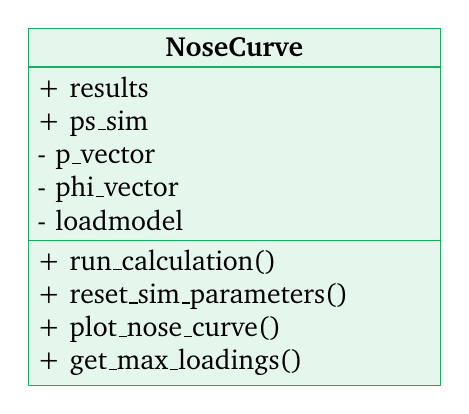
\begin{tikzpicture}
        % \footnotesize
        % \begin{package}{voltage}
            \begin{class}[text width=5cm]{NoseCurve}{0,0}
                \attribute{+ results}
                \attribute{+ ps$\_$sim}
                \attribute{- p$\_$vector}
                \attribute{- phi$\_$vector}
                \attribute{- loadmodel}
                \operation{+ run$\_$calculation()}
                \operation{+ reset$\_$sim$\_$parameters()}
                \operation{+ plot$\_$nose$\_$curve()}
                \operation{+ get$\_$max$\_$loadings()}
            \end{class}       
        % \end{package}
    \end{tikzpicture}
    \caption{Class NoseCurve Diagram}
\end{figure}

\tikzsetnextfilename{class_diagram_nosecurve_complete}
\begin{figure}[htb]
    \centering
    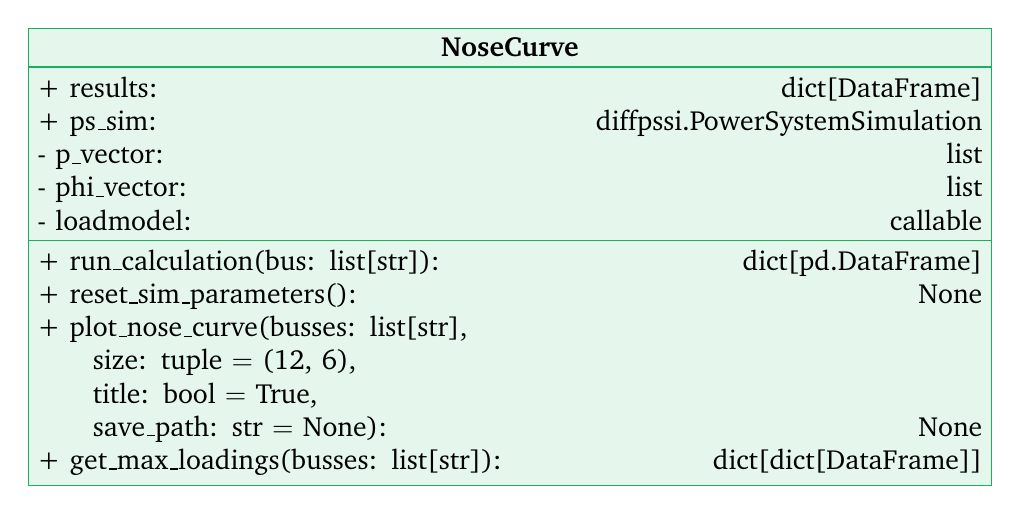
\begin{tikzpicture}
        % \footnotesize
        % \begin{package}{voltage}
            \begin{class}[text width=12cm]{NoseCurve}{0,0}
                \attribute{+ results: \hfill dict[DataFrame]}
                \attribute{+ ps$\_$sim: \hfill diffpssi.PowerSystemSimulation}
                \attribute{- p$\_$vector: \hfill list}
                \attribute{- phi$\_$vector: \hfill list}
                \attribute{- loadmodel: \hfill callable}
                \operation{+ run$\_$calculation(bus: list[str]): \hfill dict[pd.DataFrame]}
                \operation{+ reset$\_$sim$\_$parameters(): \hfill None}
                \operation{+ plot$\_$nose$\_$curve(busses: list[str],\\\quad\quad size: tuple $=$ (12, 6),\\\quad\quad title: bool $=$ True,\\\quad\quad save$\_$path: str $=$ None): \hfill None}
                \operation{+ get$\_$max$\_$loadings(busses: list[str]): \hfill dict[dict[DataFrame]]}
            \end{class}       
        % \end{package}
    \end{tikzpicture}
    \caption{Class NoseCurve Diagram Complete}
\end{figure}

\tikzsetnextfilename{class_diagram_oltc_transformer_complete}
\begin{figure}[htb]
    \centering
    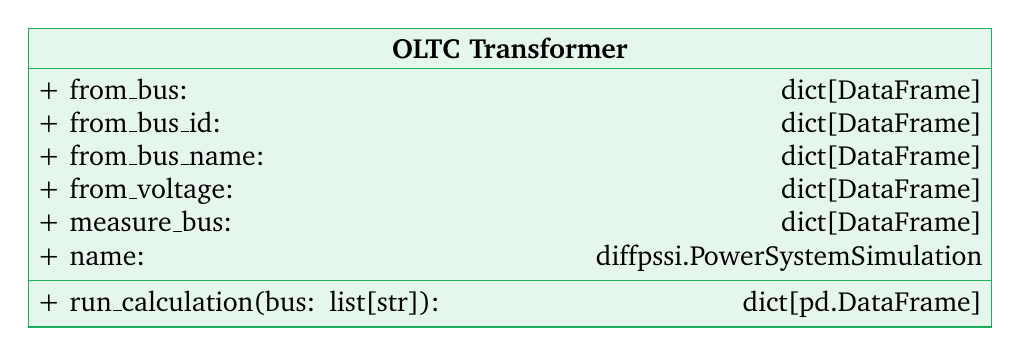
\begin{tikzpicture}
        % \footnotesize
        % \begin{package}{voltage}
            \begin{class}[text width=12cm]{OLTC Transformer}{0,0}
                \attribute{+ from$\_$bus: \hfill dict[DataFrame]}
                \attribute{+ from$\_$bus$\_$id: \hfill dict[DataFrame]}
                \attribute{+ from$\_$bus$\_$name: \hfill dict[DataFrame]}
                \attribute{+ from$\_$voltage: \hfill dict[DataFrame]}
                \attribute{+ measure$\_$bus: \hfill dict[DataFrame]}
                \attribute{+ name: \hfill diffpssi.PowerSystemSimulation}

                \operation{+ run$\_$calculation(bus: list[str]): \hfill dict[pd.DataFrame]}
            \end{class}       
        % \end{package}
    \end{tikzpicture}
    \caption{Class OLTC Transformer Diagram Complete}
\end{figure}

\begin{landscape}
    \tikzsetnextfilename{software_structure}
    \begin{figure}[htb]
        \centering
        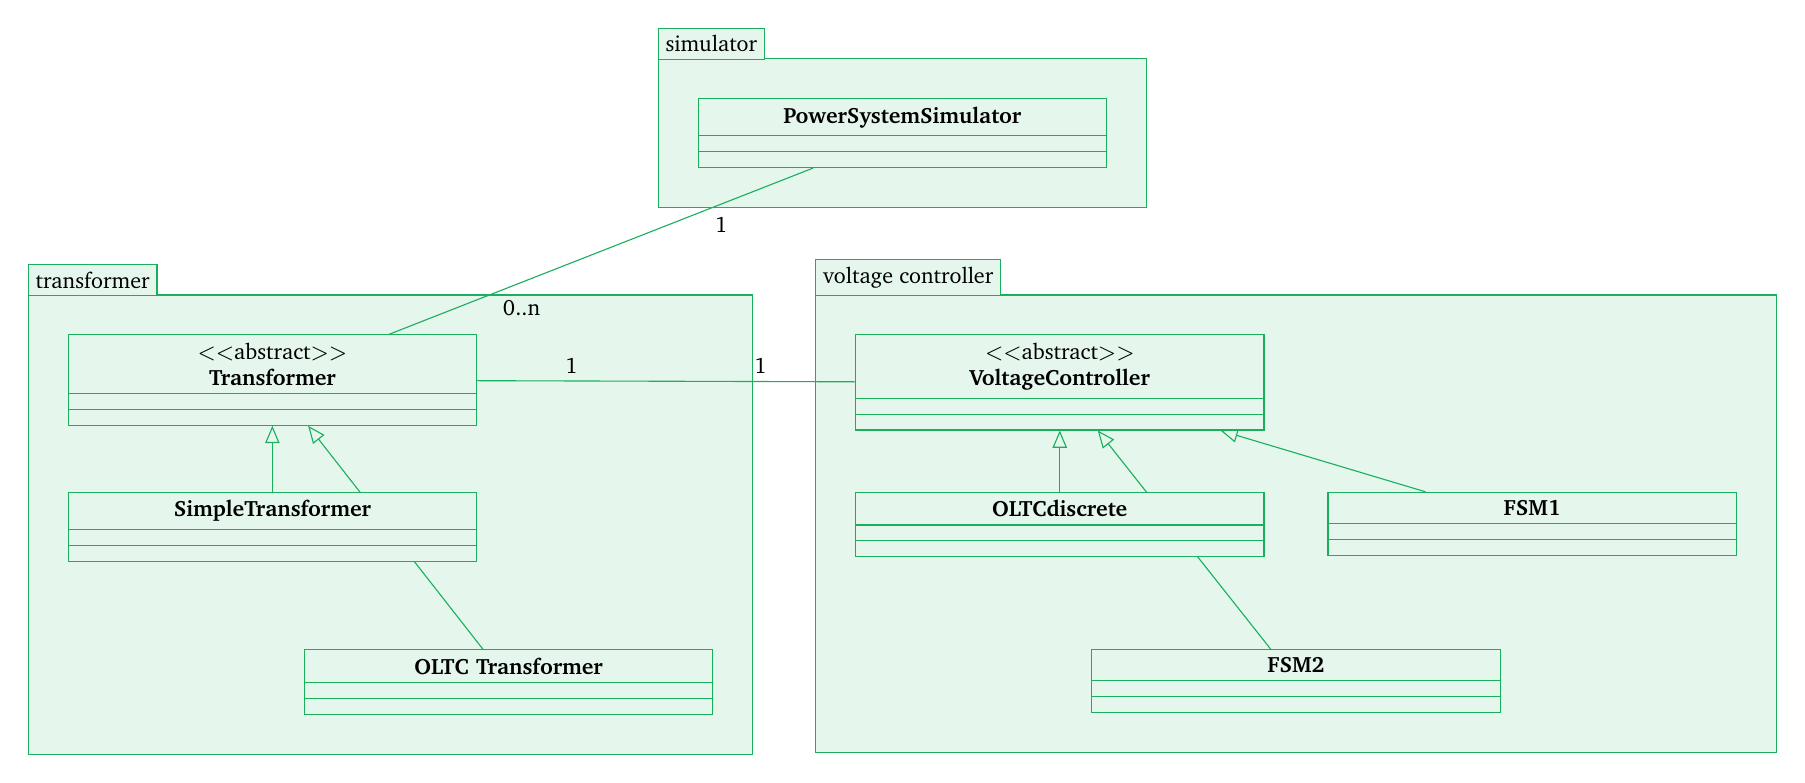
\begin{tikzpicture}% [show background grid]
            \footnotesize
            \begin{package}{simulator}
                \begin{class}{PowerSystemSimulator}{0,0}
                \end{class}       
            \end{package}
            \begin{package}{transformer}
                \begin{abstractclass}{Transformer}{-8,-3}
                \end{abstractclass}

                \begin{class}{SimpleTransformer}{-8,-5}
                    \inherit{Transformer}
                \end{class}
                \begin{class}{OLTC Transformer}{-5,-7}
                    \inherit{Transformer}
                \end{class}
            \end{package}
            \begin{package}{voltage controller}
                \begin{abstractclass}{VoltageController}{2,-3}
                \end{abstractclass}
                \begin{class}{OLTCdiscrete}{2,-5}
                    \inherit{VoltageController}
                \end{class}
                \begin{class}{FSM1}{8,-5}
                    \inherit{VoltageController}
                \end{class}
                \begin{class}{FSM2}{5,-7}
                    \inherit{VoltageController}
                \end{class}
            \end{package}

            \association{Transformer}{}{0..n}{PowerSystemSimulator}{}{1}
            \association{VoltageController}{}{1}{Transformer}{}{1}
        \end{tikzpicture}
        \caption{Software Structure idea}
    \end{figure}
\end{landscape}

% \begin{tikzpicture}[node distance = 1.5cm, auto]
%     % Place nodes
%     \node [papStart] (Start1){Start};
%     \node [papProcess, below of = Start1,label={[shift={(2.7,-0.6)}]\footnotesize\textit{label 1}}] (pro1){Prozess};
%     \node [papProcess, below of = pro1,label={[shift={(3,-0.6)}]\footnotesize\textit{label 2}}](pro2){Prozess};
%     \node [papDecision, below of = pro2, yshift= -9mm](dec1){Entscheidung};
%     \node [papPredProc,  right of = dec1, xshift=25mm](predproc1){\nodepart{two}\shortstack{vordefinierter\\Prozess}};
%     \node [papProcess, below of = predproc1,label={[shift={(2.3,-0.6)}]\footnotesize\textit{label 3}}](pro3){Prozess};
%     \node [papEnd, below of = dec1, yshift= -20mm] (End) {Ende};
    
%     % Place joins
%     \coordinate [below of = dec1, yshift= -10mm] (join1);
    
%     % Draw edges
%     \path [papLine] (Start1) -- (pro1);
%     \path [papLine] (pro1) -- (pro2);
%     \path [papLine] (pro2) -- (dec1);
%     \path [papLine] (dec1) -- node [right] {\papYes} (End);
%     \path [papLine] (dec1) -- node [above] {\papNo} (predproc1);
%     \path [papLine] (predproc1) -- (pro3);
%     \path [papLine] (pro3) |- (join1);
% \end{tikzpicture}

\end{document}